
% \documentclass{standalone}
% \input{../tikz_header}

% \begin{document}

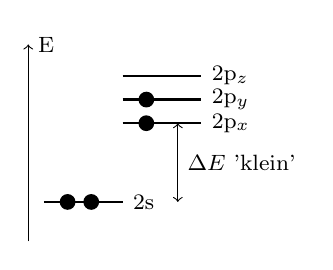
\begin{tikzpicture}[font=\footnotesize]
  


   \draw [->] (-0.2,-0.5) -- ++ (0,2.5) node [right] {E};

   \draw[thick] (0,0) -- ++ (1,0) node [right] {2s};
   \fill[black] (0.3, 0) circle (1mm);
   \fill[black] (0.6, 0) circle (1mm);

   \draw[thick] (1,1) -- ++ (1,0) node [right] {2p$_x$};
   \fill[black] (1.3, 1) circle (1mm);

   \draw[thick] (1,1.3) -- ++ (1,0) node [right] {2p$_y$};
   \fill[black] (1.3, 1.3) circle (1mm);

   \draw[thick] (1,1.6) -- ++ (1,0) node [right] {2p$_z$};


   \draw [<->] (1.7, 0) -- node[right] {$\Delta E$ 'klein'} ++ (0, 1) ;



\end{tikzpicture}

%\end{document}